% This is "sig-alternate.tex" V2.1 April 2013
% This file should be compiled with V2.5 of "sig-alternate.cls" May 2012
%
% This example file demonstrates the use of the 'sig-alternate.cls'
% V2.5 LaTeX2e document class file. It is for those submitting
% articles to ACM Conference Proceedings WHO DO NOT WISH TO
% STRICTLY ADHERE TO THE SIGS (PUBS-BOARD-ENDORSED) STYLE.
% The 'sig-alternate.cls' file will produce a similar-looking,
% albeit, 'tighter' paper resulting in, invariably, fewer pages.
%
% ----------------------------------------------------------------------------------------------------------------
% This .tex file (and associated .cls V2.5) produces:
%       1) The Permission Statement
%       2) The Conference (location) Info information
%       3) The Copyright Line with ACM data
%       4) NO page numbers
%
% as against the acm_proc_article-sp.cls file which
% DOES NOT produce 1) thru' 3) above.
%
% Using 'sig-alternate.cls' you have control, however, from within
% the source .tex file, over both the CopyrightYear
% (defaulted to 200X) and the ACM Copyright Data
% (defaulted to X-XXXXX-XX-X/XX/XX).
% e.g.
% \CopyrightYear{2007} will cause 2007 to appear in the copyright line.
% \crdata{0-12345-67-8/90/12} will cause 0-12345-67-8/90/12 to appear in the copyright line.
%
% ---------------------------------------------------------------------------------------------------------------
% This .tex source is an example which *does* use
% the .bib file (from which the .bbl file % is produced).
% REMEMBER HOWEVER: After having produced the .bbl file,
% and prior to final submission, you *NEED* to 'insert'
% your .bbl file into your source .tex file so as to provide
% ONE 'self-contained' source file.
%
% ================= IF YOU HAVE QUESTIONS =======================
% Questions regarding the SIGS styles, SIGS policies and
% procedures, Conferences etc. should be sent to
% Adrienne Griscti (griscti@acm.org)
%% Technical questions _only_ to
% Gerald Murray (murray@hq.acm.org)
% ===============================================================
%
% For tracking purposes - this is V2.0 - May 2012

\documentclass{sig-alternate-05-2015}


\begin{document}

% Copyright
\setcopyright{acmcopyright}
%\setcopyright{acmlicensed}
%\setcopyright{rightsretained}
%\setcopyright{usgov}
%\setcopyright{usgovmixed}
%\setcopyright{cagov}
%\setcopyright{cagovmixed}


% DOI
\doi{10.475/123_4}

% ISBN
\isbn{123-4567-24-567/08/06}

%Conference
\conferenceinfo{PLDI '13}{June 16--19, 2013, Seattle, WA, USA}

\acmPrice{\$15.00}

%
% --- Author Metadata here ---
\conferenceinfo{WOODSTOCK}{'97 El Paso, Texas USA}
%\CopyrightYear{2007} % Allows default copyright year (20XX) to be over-ridden - IF NEED BE.
%\crdata{0-12345-67-8/90/01}  % Allows default copyright data (0-89791-88-6/97/05) to be over-ridden - IF NEED BE.
% --- End of Author Metadata ---

\title{{\ttlit Turing Machine} Obfuscation Individual Study Report\titlenote{(Produces the permission block, and
copyright information). For use with
SIG-ALTERNATE.CLS. Supported by ACM.}}
%\subtitle{[Extended Abstract]
%\titlenote{A full version of this paper is available as
%\textit{Author's Guide to Preparing ACM SIG Proceedings Using
%\LaTeX$2_\epsilon$\ and BibTeX} at
%\texttt{www.acm.org/eaddress.htm}}}
%
% You need the command \numberofauthors to handle the 'placement
% and alignment' of the authors beneath the title.
%
% For aesthetic reasons, we recommend 'three authors at a time'
% i.e. three 'name/affiliation blocks' be placed beneath the title.
%
% NOTE: You are NOT restricted in how many 'rows' of
% "name/affiliations" may appear. We just ask that you restrict
% the number of 'columns' to three.
%
% Because of the available 'opening page real-estate'
% we ask you to refrain from putting more than six authors
% (two rows with three columns) beneath the article title.
% More than six makes the first-page appear very cluttered indeed.
%
% Use the \alignauthor commands to handle the names
% and affiliations for an 'aesthetic maximum' of six authors.
% Add names, affiliations, addresses for
% the seventh etc. author(s) as the argument for the
% \additionalauthors command.
% These 'additional authors' will be output/set for you
% without further effort on your part as the last section in
% the body of your article BEFORE References or any Appendices.

\numberofauthors{1} %  in this sample file, there are a *total*
% of EIGHT authors. SIX appear on the 'first-page' (for formatting
% reasons) and the remaining two appear in the \additionalauthors section.
%
\author{
% You can go ahead and credit any number of authors here,
% e.g. one 'row of three' or two rows (consisting of one row of three
% and a second row of one, two or three).
%
% The command \alignauthor (no curly braces needed) should
% precede each author name, affiliation/snail-mail address and
% e-mail address. Additionally, tag each line of
% affiliation/address with \affaddr, and tag the
% e-mail address with \email.
%
% 1st. author
\alignauthor
Yan Wang\titlenote{None.}\\
       \affaddr{College of Information Sciences and Technology}\\
       \affaddr{The Pennsylvania State University}\\       
       \email{ybw5084@ist.psu.edu}
}
% There's nothing stopping you putting the seventh, eighth, etc.
% author on the opening page (as the 'third row') but we ask,
% for aesthetic reasons that you place these 'additional authors'
% in the \additional authors block, viz.
%\additionalauthors{Additional authors: John Smith (The Th{\o}rv{\"a}ld Group,
%email: {\texttt{jsmith@affiliation.org}}) and Julius P.~Kumquat
%(The Kumquat Consortium, email: {\texttt{jpkumquat@consortium.net}}).}
%\date{30 July 1999}
% Just remember to make sure that the TOTAL number of authors
% is the number that will appear on the first page PLUS the
% number that will appear in the \additionalauthors section.

\maketitle
\begin{abstract}
Software obfuscation is a crucial research filed due to the severe computer security situation of Internet era. It could complicate source programs to make it difficult for attackers to do reverse engineering in this malicious codes and software vulnerabilities are constrained from spreading. In this paper we proposed a novel method to do software obfuscation. Predicates in source codes are transformed to different Turing Machine programs. Control flow graph could be complicated to a great extent by leveraging this transformation so software obfuscation is achieved. This paper records the research progress of my research project Turing Machine Obfuscation.
\end{abstract}




\keywords{Turing Machine; Software Obfuscation; Encoding; Control Flow}

\section{Introduction}
Software Obfuscation is an important cryptographic concept with wide applications\cite{lynn:positive}.However until recently there was little theoretical investigation of obfuscation, despite the great success theoretical cryptography has had in tackling other challenging notions of security. The goal of conducting software obfuscation is to hide those classified or sensitive information at the same time preserving software’s functionality. We can always treat obfuscation method as a virtual black box or a compiler which could transform the primitive source code to instrumented codes that will behave exactly the same as the original codes.  Which means, the obfuscated programs will yield outputs the same with the original outputs given identical inputs.

This Paper is organized as follows: Section 2 addresses current progress in obfuscation research domain, Section 3 states our proposed method Turing Machine in detail, in addition, current progress will be covered as well. Section 4 illustrates experiments we plan to use to  evaluate our proposal's performance, Section 5 concludes the whole paper.

\section{Related Works}
In Paper "Positive results and techniques for obfuscation"\cite{lynn:positive}, the essence of obfuscation is analyzed and several common methods for software obfuscation were brought about. Generally speaking, many cryptographic applications exist including "Intellectual  property" protection which lies in securing secret algorithms and keys, authority and access controlling and private-key and public-key encryption transformation. The authors focused on access control in this paper. This paper gave the first method for program obfuscation which was proved effective. This paper basically is a theoretical research. It didn't involve with any experiments or simulation.  Through using Oracle model, the paper proposed a method of reducing obfuscation of one family to obfuscating another. The paper illuminated the future research direction.

Paper "Waermarking, tamper-proofing, and obfuscation - tools for software protection"\cite{Collberg:wartermarking} summarized three types of software attack and corresponding technical defense methods of three main categories including obfuscation. Based on what this paper expressed, obfuscation technology is targeting reverse engineering attack. Through software obfuscation, instrumented software is still functional but unintelligible.  Watermarking is another defense category which deals with software privacy probing which could enable identification of a certain assembled software. The last technology mentioned is tamper-proofing which aims at disable the software functionalities in unauthorized copies. \cite{Collberg:wartermarking} is a typical overview journal paper which summarize current research conditions and progresses so that further research could be well-guided. We can literally take this paper as a survey of software security. 

Paper "On the Concept of Software Obfuscation in Computer Security"."On the concept of software obfuscation in computer security."\cite{Kuzurin:Onthe}  proposed that the requirements for obfuscation should not be universal but dependent on a specific  program to be obfuscated. This paper mainly talked about obfuscator's security requirements. From their perspective, it makes sense to do varies kinds of obfuscation with respect to different software security definition. In total, authors of this paper proposed five kinds of model including "black box" and "grey box" which both belongs to total obfuscation, software protection obfuscation, hiding constant obfuscation and predicate obfuscation.

Paper "Indistinguishability Obfuscation for Turing Machines with Unbounded Memory"\cite{Koppula:Indistinguishability} is a research paper very close to my research topic. The authors of this paper showed how to build indistinguishability obfuscation with modest overhead. The overhead growth was polynomial in terms of security parameter lambda and Turing machine input X. To achieve this goal, they invent a novel primitive which enable the accumulator to own a much larger memory with only a small commitment. The proposed primitive even allow different programs equivalent when they were not at the same stage. It means that this novel primitive is indistinguishability obfuscation friendly. Although this papers' research topic is very similar to mine, the research content was distinct from my Turing obfuscation research. This paper focused on theory proof taking advantage of the Turing machine as a model. However, mine research cares more about Turing encoding and obfuscation implementation and performance evaluation.

Papers above demonstrate theoretical research in obfuscation which is a very crucial part of obfuscation area. In addition, some recent papers published in conferences showed more interests in research on obfuscation implementation methods.

Paper "Translingual Obfuscation"\cite{Wang:Translingual} is a paper of such kind. "Translingual" is a new term invented by the authors of this paper. The basic idea behind this term is to convert programs' language from one to another in order to achieve obfuscation effect. Through the "misusing" of the semantics and syntax of a certain programming language, input source program could easily become much more complicated. In particular, this translingual method only transform a portion of source codes which technically made a mix of two or more programming language. In this paper, the authors used Prolog as the target language and C language as the source language. The reason for this Prolog choice may come from its complicated syntax which could make translingual obfuscation more powerful.  Prolog's two feature: unification and backtracking were used to make an obfuscation tool called "BABEL". In this way BABEL obfuscation tool could provide effective and stealthy obfuscation. The authors also did lots of experiments to measure the effectiveness of "BABEL". BABEL proved to be superior to common used commodity obfuscation tool in terms of four traditional bench marks used for evaluation obfuscation performance: Potency, Resilience, Cost and Stealth.

In paper "Control flow obfuscation with information flow tracking"\cite{Chen:Control}, the authors proposed a novel application of information flow tracking which has been widely used in securing software execution with only a modest overhead during program execution. This paper took advantage of two key features which are called "the architectural support for automatic propagation of tags" and "violation handling of tag misuses" in information flow tracking area\cite{Chen:Control}. The novelty in this paper lies in the tag usage. They use the tags during propagation as a flow sensitive predicates in order to hide normal control flow transfers. Which means the real control flow transfer happens at the same time tags are leveraged as predicates for control flow transferred to the violation handler. Further experiments were conducted to test the effectiveness of this method and the experiment results showed that their proposed scheme "BOSH" indeed could obfuscate the whole control flow with minor overhead added.

There are several techniques to protect sensitive information in software including obfuscation, encryption, partial server-side execution and trusted native code\cite{Collberg:Ataxonomy}, which is expressed by figure 1. In this paper, authors argued that automatic code obfuscation is the most promising method with respect to potency, resilience and cost. The main contribution of this paper is the proposed insight that it is acceptable and normal for obfuscated programs to behave differently than the original source codes. Which means that instrumented codes should run slower and be larger. As long as the observable behavior experienced by a user of this original and obfuscated pair is identical, the purpose of obfuscation is achieved.
\begin{figure}
\centering
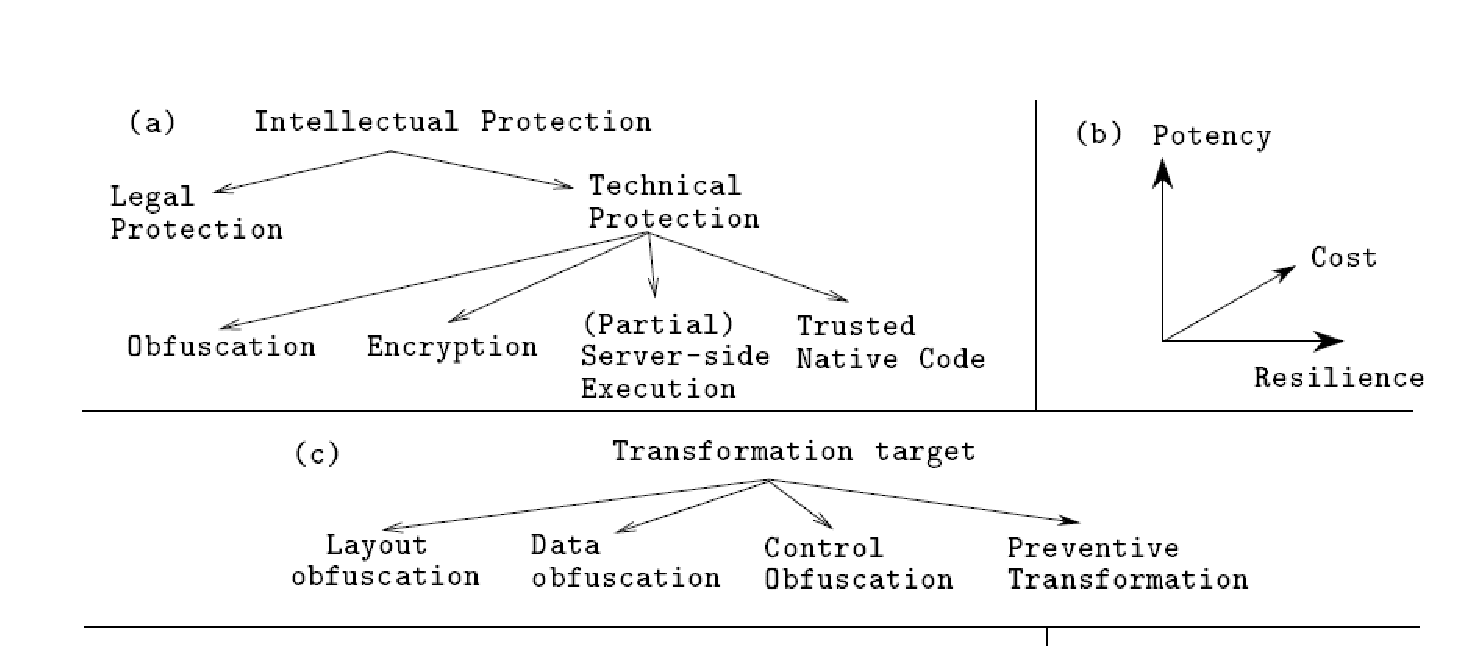
\includegraphics[width=0.5\textwidth]{taxnomy1}
\caption{Taxonomy of Intellectual Protection}
\end{figure}

Paper "Deobfuscation of Virtualization-Obfuscated Software"\cite{Coogan:Deobfuscation} focused more on de-obfuscating malware. The most common reverse engineer model is to reverse code interpreter first and then based on the accomplishment to figure out program's control flow and algorithm logic. However, this model can not be applied to all cases. This paper's main contribution lied on the proposition of a new approach which identified instructions that could affect those observable behavior of the obfuscated code. Unlike traditional outside-in reversing method, this inside-out approach requires fewer assumptions so the domain of cased eligible for obfuscation would be broadened. Results of deobfuscation malicious code are good.

Book "Reversing: secrets of reverse engineering"\cite{Eilam:Reversing} is a good tutorial for doing obfuscation. I read chapter one of this book. Chapter one clarified the concept of reverse engineering. More details about reversing were illustrated in the first chapter. Security related reversing, reversing cryptographic algorithms, program binary auditing, reversing development in software and how to achieve interoperability with proprietary software were introduced also.	
\section{Research Method}
\subsection{Turing Machine}
A Turing Machine is an abstract mathematic computation model which is named after British scientist Alan Turing. This abstract machine model simulates the behavior of a strip of tape under control of a serious of transition rules. There are several components in a Turing Machine such as a header which could read and write on tape(Figure 2) , a transition table (Figure 3)which designates the transformation rules, a state register that could record the current state of Turing machine. We could see that any combination of Turing Machine state and tape symbol corresponds to a entry of this transition table which is also represented by a 5 item tuple. A Turing Machine will always work based on the instruction tuple rules to decide which direction to go, what symbol to write and which state to enter . The basic idea for inventing this Turing machine is to convert any logic problem to a Turing Machine mathematical problem. With the help of a Turing Machine, two famous questions could be answered explicitly. 1. Does a machine exist that can figure out that whether a machine conduction on a tape involves with a loop which means the machine can't stop. 2. Is there a machine which could determine whether any arbitrary machine on its tape can eventually print one of the given symbols. Thus, the computability could be demonstrated by operation a Turing Machine. This is significant because any algorithm's logic could be simulated through operating a Turing Machine despite its extreme simplicity.
\begin{figure}
\centering
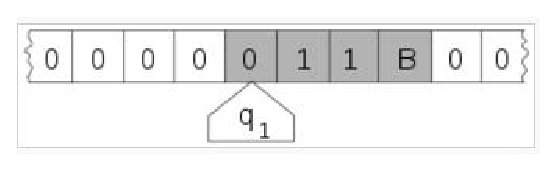
\includegraphics[width=0.4\textwidth]{tape}
\caption{ A \texttt{Turing Machine} tape.}
\end{figure}

\begin{figure}
\centering
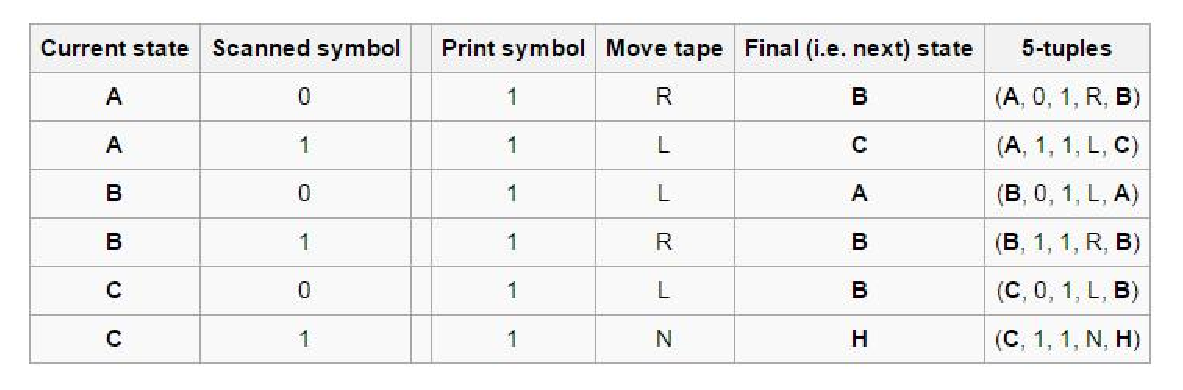
\includegraphics[width=0.4\textwidth]{TM_Table}
\caption{ A \texttt{Turing Machine} Transition Table.}
\end{figure}



\subsection{Universal Turing Machine}
Universal Turing Machine(Figure 4) is a special Turing Machine which could simulate multiple arbitrary Turing machine execution.  Every Turing machine computes a certain fixed partial computable function from the input strings over its alphabet. In that sense it behaves like a computer with a fixed program\cite{WEB:UTM}. Universal Turing machine could encode any action table in string at the same time constructing a tape which delineates input parameters. Hence, a universal Turing machine could obtain arbitrary Turing machine computation results combining the action table encoding and input table construction. Universal Turing Machine could be taken as an interpreter of a specific Turing Machine.
\begin{figure}
\centering
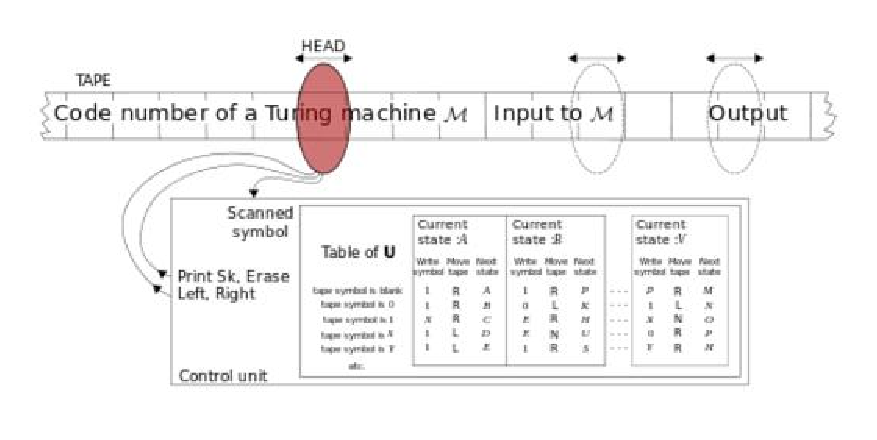
\includegraphics[width=0.4\textwidth]{UTM}
\caption{\texttt{Universal Turing Machine} }
\end{figure}

\subsection{Turing Machine Encoding}
We know that every piece of program could be transformed to a Turing Machine fulfilling the same functionality. The fact is that we don't need to change every line of source program to do the obfuscation. We are particularly interested in some operators that involve with the control flow graph of the whole program such as '+', '-','*','/','>','<','==' and so on. In our research proposal, we plan to extract all these "special" operators from the source codes and use Universal Turing Machine to encode all the predicate codes and arithmetic code part. In this way, we could decide which direction to go based on the final state of a Turing Machine. Hence, target program would be obfuscated with our Turing encoding and reverse engineering is complicated to a great extent or even made impossible.
\subsection{Current Progress}
To make our research plan more applicable and more detailed, we have divided this project into several sections.
\begin{enumerate}  
\item Construct Turing Machine prototype including all components such as tape, transition table etc.
\item Contruct Universal Turing Machine
\item Implement all operators like '+','-' and so on
\item Replace all integer expressions which used these operators with different Universal Turing Machine in source code
\item Run a large volume of experiments to test our method
\end{enumerate}

For now, we have finished to first two steps of the whole process and are implementing all the target operators with Turing Machine.


\section{Experiment Design}
There are several common benchmarks used to measure the performance of a obfuscation method: potency,resilience,cost and stealth. We decide to leverage these benchmarks to describe our Turing Machine obfuscation quantitatively. Besides this,in every aspect of evaluation, we need a commonly used obfuscation technology to compare our proposed Turing Obfuscation with. Code Virtualizer(CV) is a commonly used commercial obfuscator. We will compare Turing obfuscation performance with CV obfuscation performance.
\subsection{Potency}
Basically potency is a index of how powerful a certain obfuscation method is. Some program attributes could indicate this benchmark such as the number of Call Graph Edges(CGF), number of Control Flow Graph(CFG) edges, number of basic blocks in the program, cyclomatic number and knot count. Intuitively, the bigger the number of these attributes is, the more complicated a program is and the stronger a obfuscation method is accordingly. These metrics have been used to measure obfuscation performance in academia. So potency will be measured in terms of these attributes and through the comparison between ours and target obfuscation method.
\begin{figure}
\centering
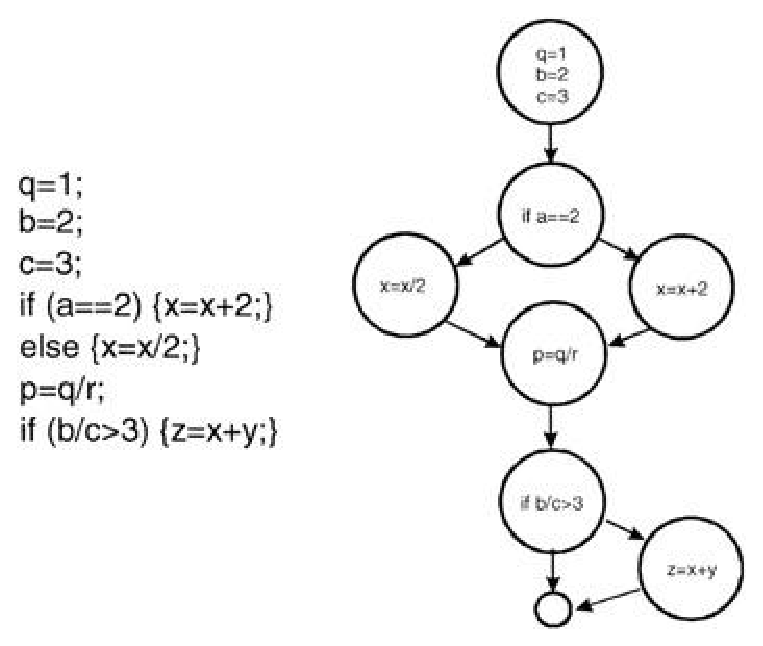
\includegraphics[width=0.45\textwidth]{CFG}
\caption
{
\texttt{Control Flow Graph Example.} 
\texttt{Source:A Practitioners Guide to Software Test Design:Chapter 10}
}

\end{figure}

\subsection{}
\subsection{Type Changes and {\subsecit Special} Characters}
We have already seen several typeface changes in this sample.  You
can indicate italicized words or phrases in your text with
the command \texttt{{\char'134}textit}; emboldening with the
command \texttt{{\char'134}textbf}
and typewriter-style (for instance, for computer code) with
\texttt{{\char'134}texttt}.  But remember, you do not
have to indicate typestyle changes when such changes are
part of the \textit{structural} elements of your
article; for instance, the heading of this subsection will
be in a sans serif\footnote{A third footnote, here.
Let's make this a rather short one to
see how it looks.} typeface, but that is handled by the
document class file. Take care with the use
of\footnote{A fourth, and last, footnote.}
the curly braces in typeface changes; they mark
the beginning and end of
the text that is to be in the different typeface.

You can use whatever symbols, accented characters, or
non-English characters you need anywhere in your document;
you can find a complete list of what is
available in the \textit{\LaTeX\
User's Guide}\cite{Lamport:LaTeX}.

\subsection{Math Equations}
You may want to display math equations in three distinct styles:
inline, numbered or non-numbered display.  Each of
the three are discussed in the next sections.

\subsubsection{Inline (In-text) Equations}
A formula that appears in the running text is called an
inline or in-text formula.  It is produced by the
\textbf{math} environment, which can be
invoked with the usual \texttt{{\char'134}begin. . .{\char'134}end}
construction or with the short form \texttt{\$. . .\$}. You
can use any of the symbols and structures,
from $\alpha$ to $\omega$, available in
\LaTeX\cite{Lamport:LaTeX}; this section will simply show a
few examples of in-text equations in context. Notice how
this equation: \begin{math}\lim_{n\rightarrow \infty}x=0\end{math},
set here in in-line math style, looks slightly different when
set in display style.  (See next section).

\subsubsection{Display Equations}
A numbered display equation -- one set off by vertical space
from the text and centered horizontally -- is produced
by the \textbf{equation} environment. An unnumbered display
equation is produced by the \textbf{displaymath} environment.

Again, in either environment, you can use any of the symbols
and structures available in \LaTeX; this section will just
give a couple of examples of display equations in context.
First, consider the equation, shown as an inline equation above:
\begin{equation}\lim_{n\rightarrow \infty}x=0\end{equation}
Notice how it is formatted somewhat differently in
the \textbf{displaymath}
environment.  Now, we'll enter an unnumbered equation:
\begin{displaymath}\sum_{i=0}^{\infty} x + 1\end{displaymath}
and follow it with another numbered equation:
\begin{equation}\sum_{i=0}^{\infty}x_i=\int_{0}^{\pi+2} f\end{equation}
just to demonstrate \LaTeX's able handling of numbering.

\subsection{Citations}
Citations to articles \cite{bowman:reasoning,
clark:pct, braams:babel, herlihy:methodology},
conference proceedings \cite{clark:pct} or
books \cite{salas:calculus, Lamport:LaTeX} listed
in the Bibliography section of your
article will occur throughout the text of your article.
You should use BibTeX to automatically produce this bibliography;
you simply need to insert one of several citation commands with
a key of the item cited in the proper location in
the \texttt{.tex} file \cite{Lamport:LaTeX}.
The key is a short reference you invent to uniquely
identify each work; in this sample document, the key is
the first author's surname and a
word from the title.  This identifying key is included
with each item in the \texttt{.bib} file for your article.

The details of the construction of the \texttt{.bib} file
are beyond the scope of this sample document, but more
information can be found in the \textit{Author's Guide},
and exhaustive details in the \textit{\LaTeX\ User's
Guide}\cite{Lamport:LaTeX}.

This article shows only the plainest form
of the citation command, using \texttt{{\char'134}cite}.
This is what is stipulated in the SIGS style specifications.
No other citation format is endorsed or supported.

\subsection{Tables}
Because tables cannot be split across pages, the best
placement for them is typically the top of the page
nearest their initial cite.  To
ensure this proper ``floating'' placement of tables, use the
environment \textbf{table} to enclose the table's contents and
the table caption.  The contents of the table itself must go
in the \textbf{tabular} environment, to
be aligned properly in rows and columns, with the desired
horizontal and vertical rules.  Again, detailed instructions
on \textbf{tabular} material
is found in the \textit{\LaTeX\ User's Guide}.

Immediately following this sentence is the point at which
Table 1 is included in the input file; compare the
placement of the table here with the table in the printed
dvi output of this document.

\begin{table}
\centering
\caption{Frequency of Special Characters}
\begin{tabular}{|c|c|l|} \hline
Non-English or Math&Frequency&Comments\\ \hline
\O & 1 in 1,000& For Swedish names\\ \hline
$\pi$ & 1 in 5& Common in math\\ \hline
\$ & 4 in 5 & Used in business\\ \hline
$\Psi^2_1$ & 1 in 40,000& Unexplained usage\\
\hline\end{tabular}
\end{table}

To set a wider table, which takes up the whole width of
the page's live area, use the environment
\textbf{table*} to enclose the table's contents and
the table caption.  As with a single-column table, this wide
table will ``float" to a location deemed more desirable.
Immediately following this sentence is the point at which
Table 2 is included in the input file; again, it is
instructive to compare the placement of the
table here with the table in the printed dvi
output of this document.


\begin{table*}
\centering
\caption{Some Typical Commands}
\begin{tabular}{|c|c|l|} \hline
Command&A Number&Comments\\ \hline
\texttt{{\char'134}alignauthor} & 100& Author alignment\\ \hline
\texttt{{\char'134}numberofauthors}& 200& Author enumeration\\ \hline
\texttt{{\char'134}table}& 300 & For tables\\ \hline
\texttt{{\char'134}table*}& 400& For wider tables\\ \hline\end{tabular}
\end{table*}
% end the environment with {table*}, NOTE not {table}!

\subsection{Figures}
Like tables, figures cannot be split across pages; the
best placement for them
is typically the top or the bottom of the page nearest
their initial cite.  To ensure this proper ``floating'' placement
of figures, use the environment
\textbf{figure} to enclose the figure and its caption.

This sample document contains examples of \textbf{.eps} files to be
displayable with \LaTeX.  If you work with pdf\LaTeX, use files in the
\textbf{.pdf} format.  Note that most modern \TeX\ system will convert
\textbf{.eps} to \textbf{.pdf} for you on the fly.  More details on
each of these is found in the \textit{Author's Guide}.

\begin{figure}
\centering
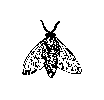
\includegraphics{fly}
\caption{A sample black and white graphic.}
\end{figure}

\begin{figure}
\centering
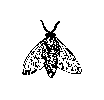
\includegraphics[height=1in, width=1in]{fly}
\caption{A sample black and white graphic
that has been resized with the \texttt{includegraphics} command.}
\end{figure}


As was the case with tables, you may want a figure
that spans two columns.  To do this, and still to
ensure proper ``floating'' placement of tables, use the environment
\textbf{figure*} to enclose the figure and its caption.
and don't forget to end the environment with
{figure*}, not {figure}!

\begin{figure*}
\centering
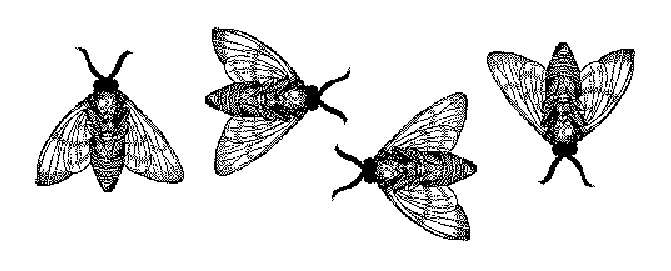
\includegraphics{flies}
\caption{A sample black and white graphic
that needs to span two columns of text.}
\end{figure*}


\begin{figure}
\centering
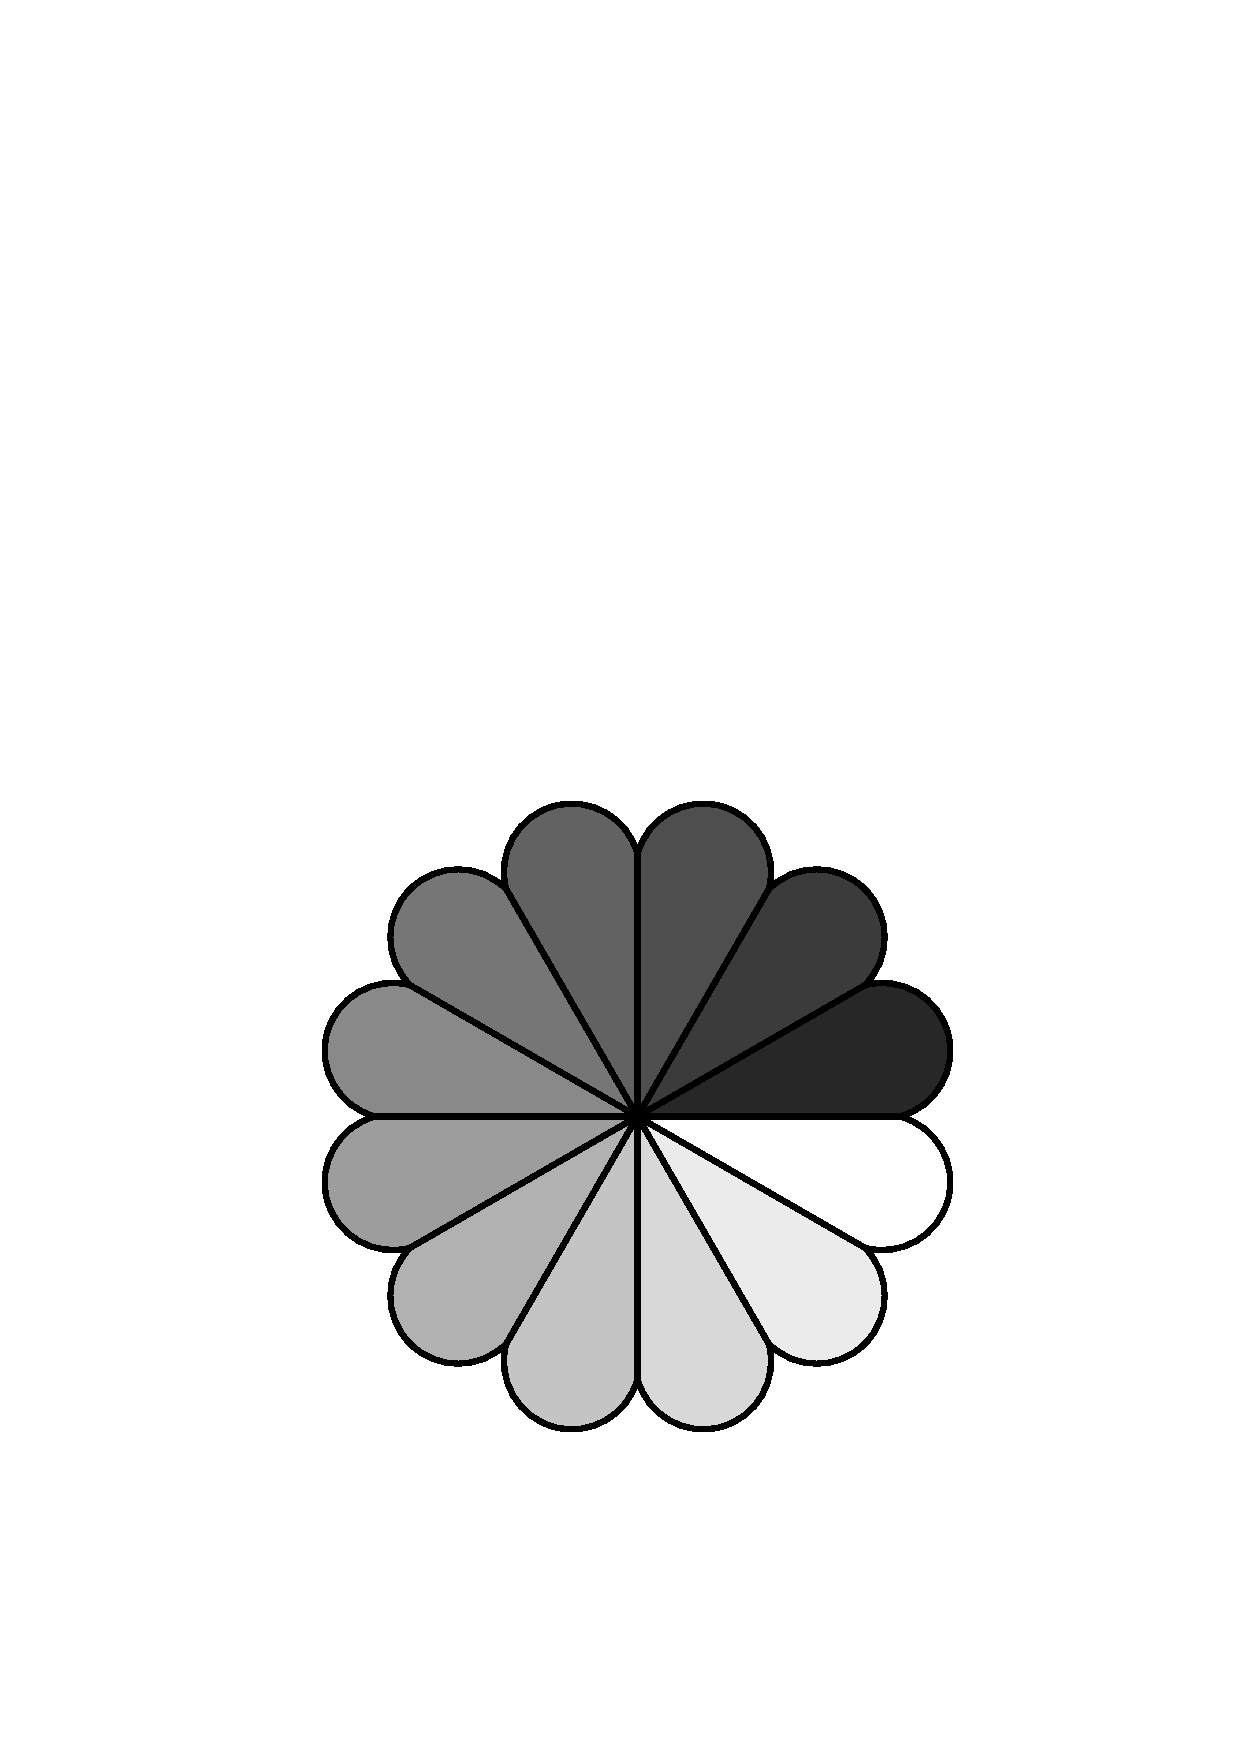
\includegraphics[height=1in, width=1in]{rosette}
\caption{A sample black and white graphic that has
been resized with the \texttt{includegraphics} command.}
\vskip -6pt
\end{figure}

\subsection{Theorem-like Constructs}
Other common constructs that may occur in your article are
the forms for logical constructs like theorems, axioms,
corollaries and proofs.  There are
two forms, one produced by the
command \texttt{{\char'134}newtheorem} and the
other by the command \texttt{{\char'134}newdef}; perhaps
the clearest and easiest way to distinguish them is
to compare the two in the output of this sample document:

This uses the \textbf{theorem} environment, created by
the\linebreak\texttt{{\char'134}newtheorem} command:
\newtheorem{theorem}{Theorem}
\begin{theorem}
Let $f$ be continuous on $[a,b]$.  If $G$ is
an antiderivative for $f$ on $[a,b]$, then
\begin{displaymath}\int^b_af(t)dt = G(b) - G(a).\end{displaymath}
\end{theorem}

The other uses the \textbf{definition} environment, created
by the \texttt{{\char'134}newdef} command:
\newdef{definition}{Definition}
\begin{definition}
If $z$ is irrational, then by $e^z$ we mean the
unique number which has
logarithm $z$: \begin{displaymath}{\log e^z = z}\end{displaymath}
\end{definition}

Two lists of constructs that use one of these
forms is given in the
\textit{Author's  Guidelines}.
 
There is one other similar construct environment, which is
already set up
for you; i.e. you must \textit{not} use
a \texttt{{\char'134}newdef} command to
create it: the \textbf{proof} environment.  Here
is a example of its use:
\begin{proof}
Suppose on the contrary there exists a real number $L$ such that
\begin{displaymath}
\lim_{x\rightarrow\infty} \frac{f(x)}{g(x)} = L.
\end{displaymath}
Then
\begin{displaymath}
l=\lim_{x\rightarrow c} f(x)
= \lim_{x\rightarrow c}
\left[ g{x} \cdot \frac{f(x)}{g(x)} \right ]
= \lim_{x\rightarrow c} g(x) \cdot \lim_{x\rightarrow c}
\frac{f(x)}{g(x)} = 0\cdot L = 0,
\end{displaymath}
which contradicts our assumption that $l\neq 0$.
\end{proof}

Complete rules about using these environments and using the
two different creation commands are in the
\textit{Author's Guide}; please consult it for more
detailed instructions.  If you need to use another construct,
not listed therein, which you want to have the same
formatting as the Theorem
or the Definition\cite{salas:calculus} shown above,
use the \texttt{{\char'134}newtheorem} or the
\texttt{{\char'134}newdef} command,
respectively, to create it.

\subsection*{A {\secit Caveat} for the \TeX\ Expert}
Because you have just been given permission to
use the \texttt{{\char'134}newdef} command to create a
new form, you might think you can
use \TeX's \texttt{{\char'134}def} to create a
new command: \textit{Please refrain from doing this!}
Remember that your \LaTeX\ source code is primarily intended
to create camera-ready copy, but may be converted
to other forms -- e.g. HTML. If you inadvertently omit
some or all of the \texttt{{\char'134}def}s recompilation will
be, to say the least, problematic.

\section{Conclusions}
This paragraph will end the body of this sample document.
Remember that you might still have Acknowledgments or
Appendices; brief samples of these
follow.  There is still the Bibliography to deal with; and
we will make a disclaimer about that here: with the exception
of the reference to the \LaTeX\ book, the citations in
this paper are to articles which have nothing to
do with the present subject and are used as
examples only.
%\end{document}  % This is where a 'short' article might terminate

%ACKNOWLEDGMENTS are optional
\section{Acknowledgments}
This section is optional; it is a location for you
to acknowledge grants, funding, editing assistance and
what have you.  In the present case, for example, the
authors would like to thank Gerald Murray of ACM for
his help in codifying this \textit{Author's Guide}
and the \textbf{.cls} and \textbf{.tex} files that it describes.

%
% The following two commands are all you need in the
% initial runs of your .tex file to
% produce the bibliography for the citations in your paper.
\bibliographystyle{abbrv}
\bibliography{sigproc}  % sigproc.bib is the name of the Bibliography in this case
% You must have a proper ".bib" file
%  and remember to run:
% latex bibtex latex latex
% to resolve all references
%
% ACM needs 'a single self-contained file'!
%
%APPENDICES are optional
%\balancecolumns
\appendix
%Appendix A
\section{Headings in Appendices}
The rules about hierarchical headings discussed above for
the body of the article are different in the appendices.
In the \textbf{appendix} environment, the command
\textbf{section} is used to
indicate the start of each Appendix, with alphabetic order
designation (i.e. the first is A, the second B, etc.) and
a title (if you include one).  So, if you need
hierarchical structure
\textit{within} an Appendix, start with \textbf{subsection} as the
highest level. Here is an outline of the body of this
document in Appendix-appropriate form:
\subsection{Introduction}
\subsection{The Body of the Paper}
\subsubsection{Type Changes and  Special Characters}
\subsubsection{Math Equations}
\paragraph{Inline (In-text) Equations}
\paragraph{Display Equations}
\subsubsection{Citations}
\subsubsection{Tables}
\subsubsection{Figures}
\subsubsection{Theorem-like Constructs}
\subsubsection*{A Caveat for the \TeX\ Expert}
\subsection{Conclusions}
\subsection{Acknowledgments}
\subsection{Additional Authors}
This section is inserted by \LaTeX; you do not insert it.
You just add the names and information in the
\texttt{{\char'134}additionalauthors} command at the start
of the document.
\subsection{References}
Generated by bibtex from your ~.bib file.  Run latex,
then bibtex, then latex twice (to resolve references)
to create the ~.bbl file.  Insert that ~.bbl file into
the .tex source file and comment out
the command \texttt{{\char'134}thebibliography}.
% This next section command marks the start of
% Appendix B, and does not continue the present hierarchy
\section{More Help for the Hardy}
The sig-alternate.cls file itself is chock-full of succinct
and helpful comments.  If you consider yourself a moderately
experienced to expert user of \LaTeX, you may find reading
it useful but please remember not to change it.
%\balancecolumns % GM June 2007
% That's all folks!
\end{document}
